\subsection{شبیه‌سازی کانال رول استند در حضور کنترل‌کننده LQR}\label{roll_lqr_section}
در بخش
\ref{quadchanell_roll}
شبیه‌سازی کانال رول استند چهارپره انجام شد. در این بخش به بررسی عملکرد چهارپره در حضور کنترل‌کننده LQR پرداخته می‌شود. در شبیه‌سازی برای بهینه‌سازی ضرایب وزنی از روش
TCACS \cite{Karimi2010}
استفاده شده است.
\begin{figure}[H]\label{lqr_roll_fig}
	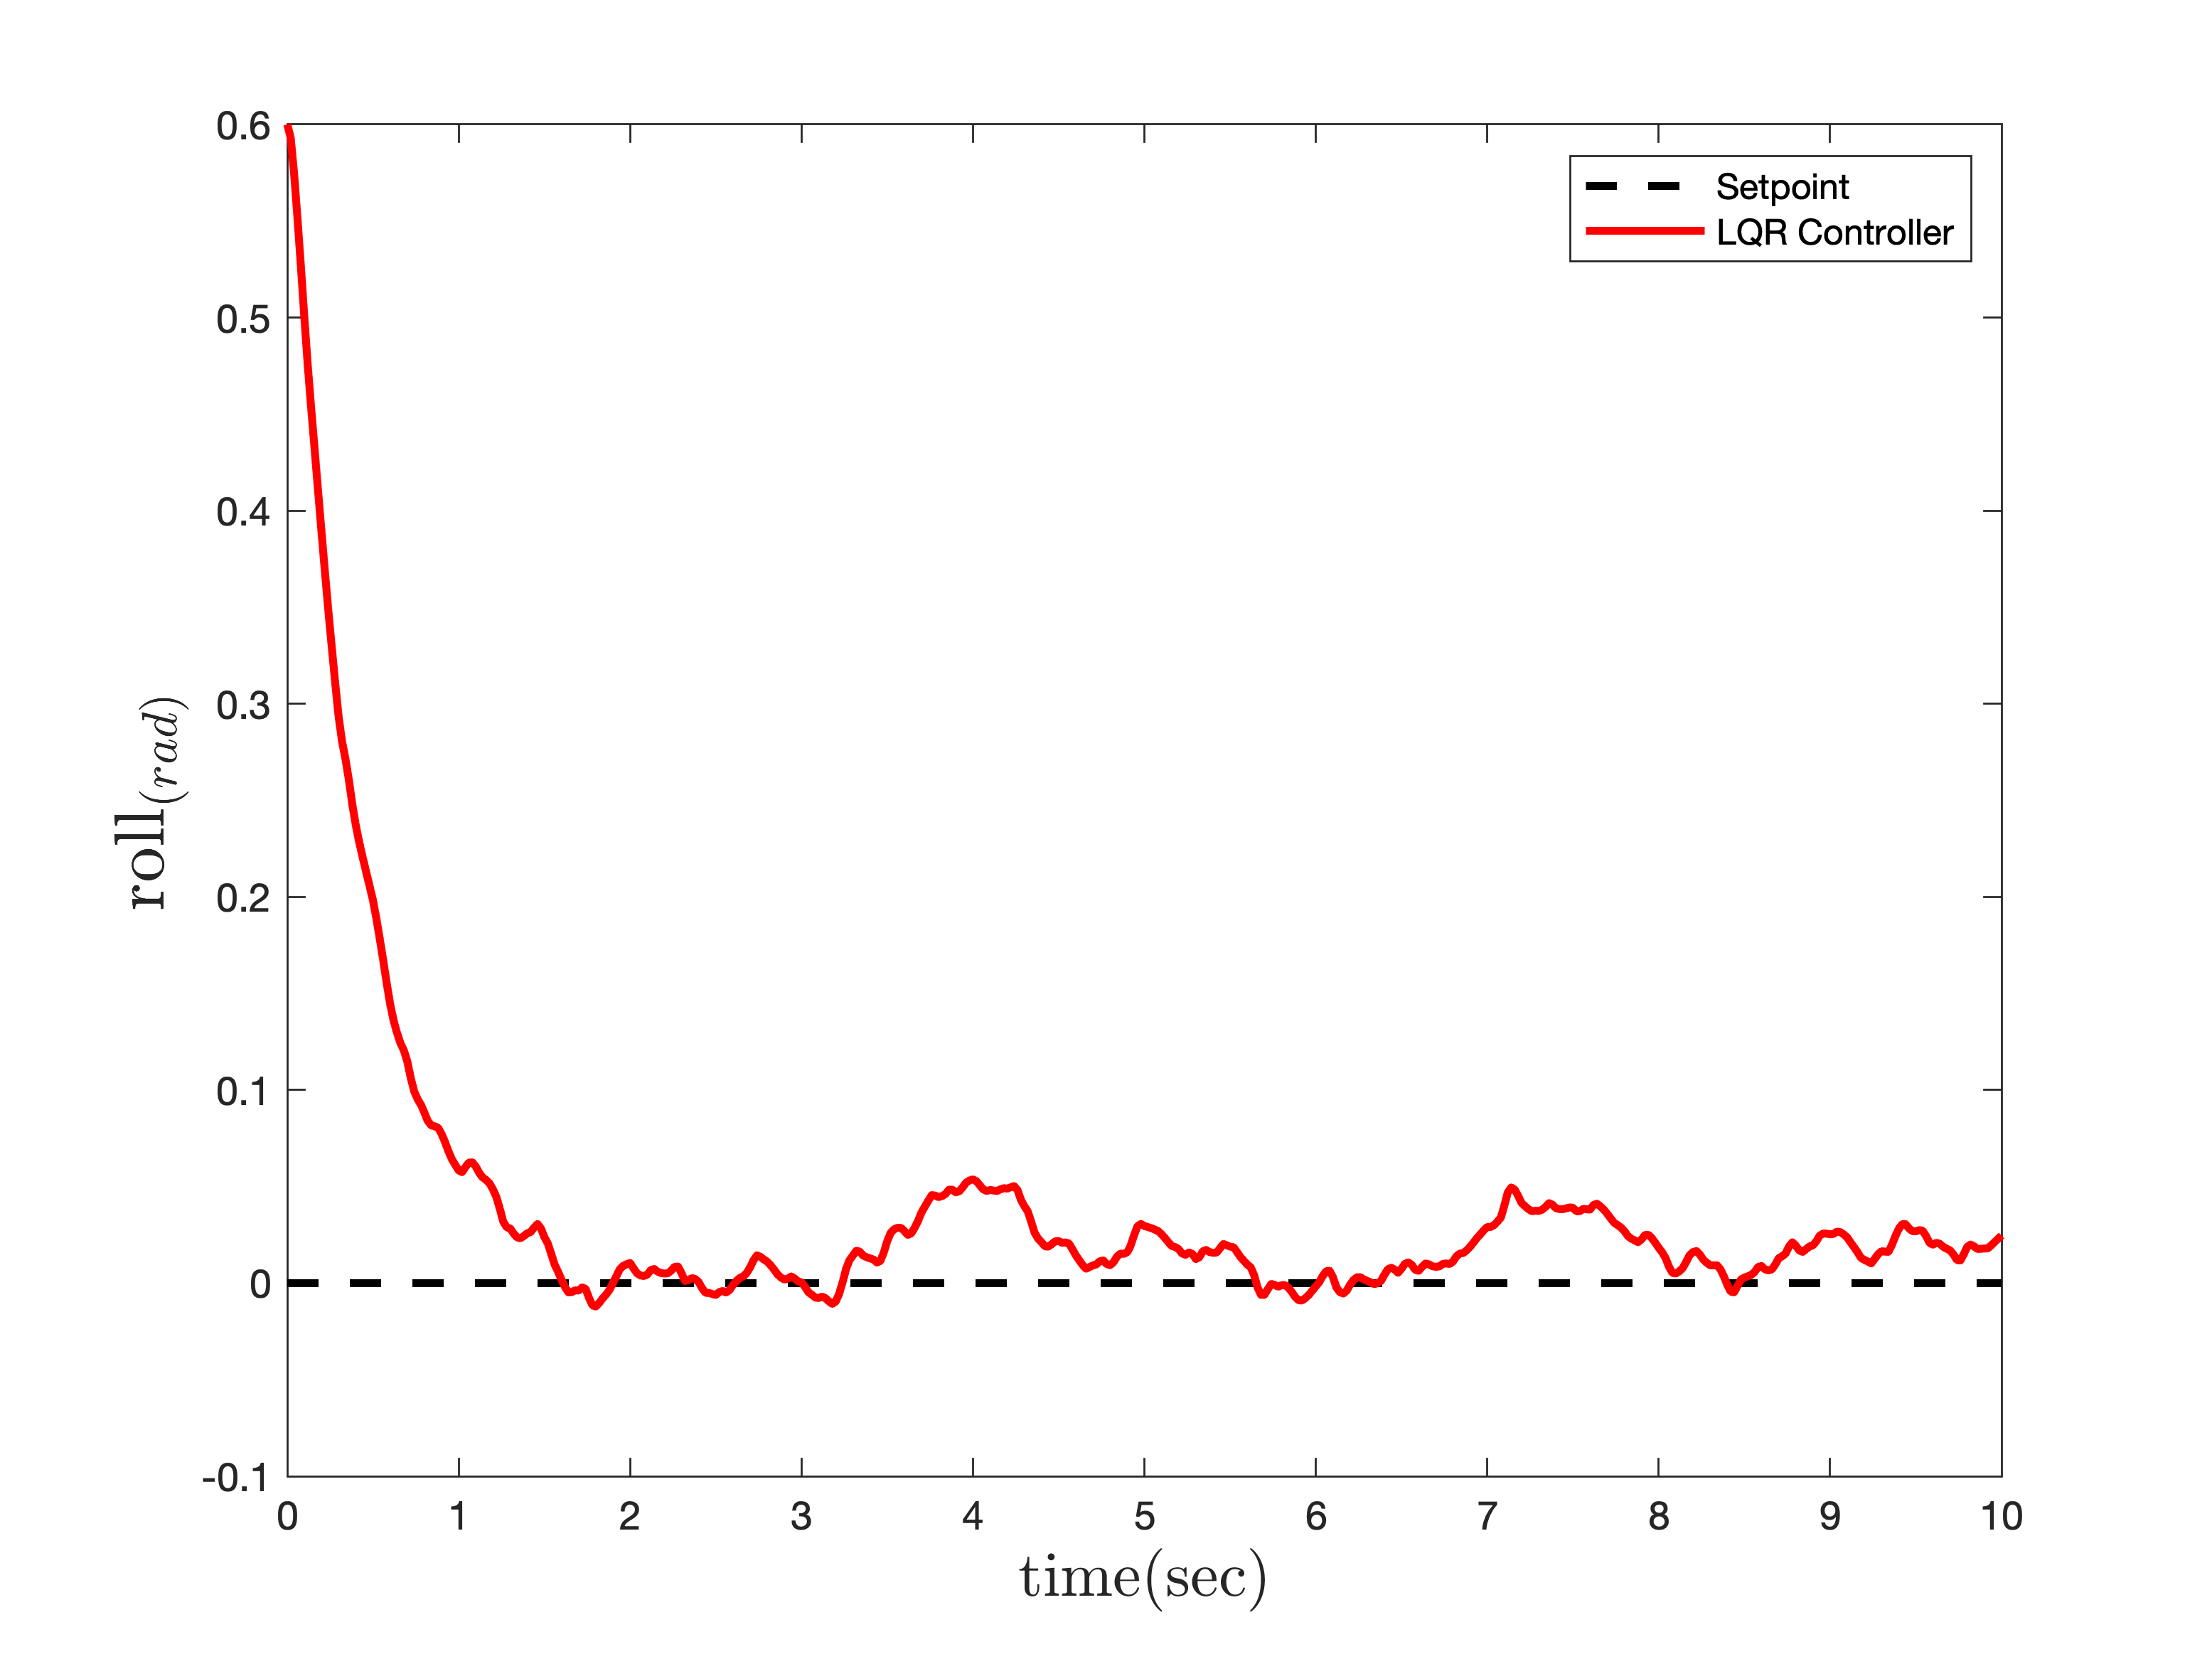
\includegraphics[width=12cm]{../Figures/MIL/LQR/Roll/lqr_roll.png}
	\centering
	\caption{عملكرد LQR در کنترل زاويه رول (تعقیب ورودی صفر)}
\end{figure}
بر اساس خروجی شبیه‌سازی (شکل
\ref{lqr_roll_fig})
،کانال رول در حضور کنترل‌کننده LQR در حدود پنج ثانیه به تعادل می‌رسد اما دارای خطای ماندگار است. 